\subsection{Case Study 3: MySQL}
\vspace{10pt}

%\mm{

MySQL is an extremely popular ACID SQL database server, the backbone of numerous commercial applications.  For our testing we deployed MySQL %was deployed 
using Amazon Relational Database Service (Amazon RDS)~\cite{amazon-rds}, which abstracts away the deployment and administration of OS and relationship database software.  We benchmark MySQL %was tested 
on the six VM types listed in Table \ref{table:awstypes}.  %Unlike for the previous case studies, we test using YCSB Workload A (50\% read, 50\% write) with a uniform distribution.

The MySQL data shows a higher variation in latency than our other case studies, and our linear regression model does not fit it as well as it does the previous two applications. %did not a linear regression as well as the first two.  
We show a sample %Example 
result for MySQL in Figure \ref{figure:mysql}. We do continue to see that the model accuracy as captured by $R^2_{predicted}$ does continue to improve with the addition of more VM types to the training set, although the value of $R^2_{predicted}$ is lower than observed for Redis and Cassandra. 

This may be due to the higher write latency of SQL databases, or possibly something with Amazon's RDS architecture that made our YCSB testing method unsuitable.  Another possibility is that the network availability for RDS varies over time, making consistent results harder to reproduce. This requires further investigation that forms part of our future work. Despite these inadequacies in our modeling, however, the basic expectation we have regarding the role of diversity does appear to hold. 
%}

  \begin{figure}
    \centering
    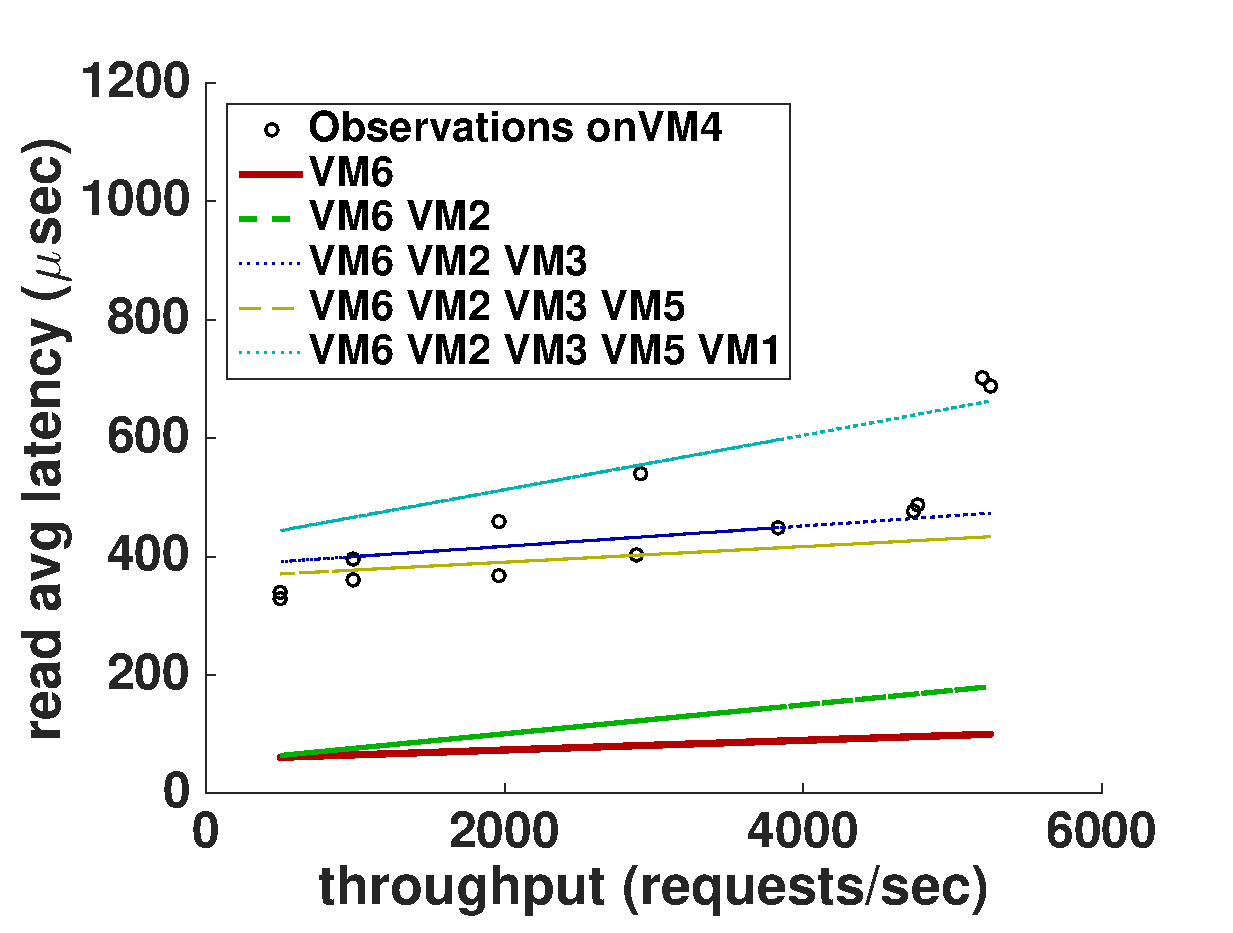
\includegraphics[scale = 0.4]{mysql_fit_read_avg_latency.eps}
    \caption{Read latency/throughput plot for MySQL. Although our multiple linear regression model offers a poorer prediction for MySQL than for our other case studies, we continue to observe an improvement in its efficacy upon increasing the diversity of the training set. }
    \label{figure:mysql}
  \end{figure}

\begin{comment}
  \begin{figure}
    \centering
    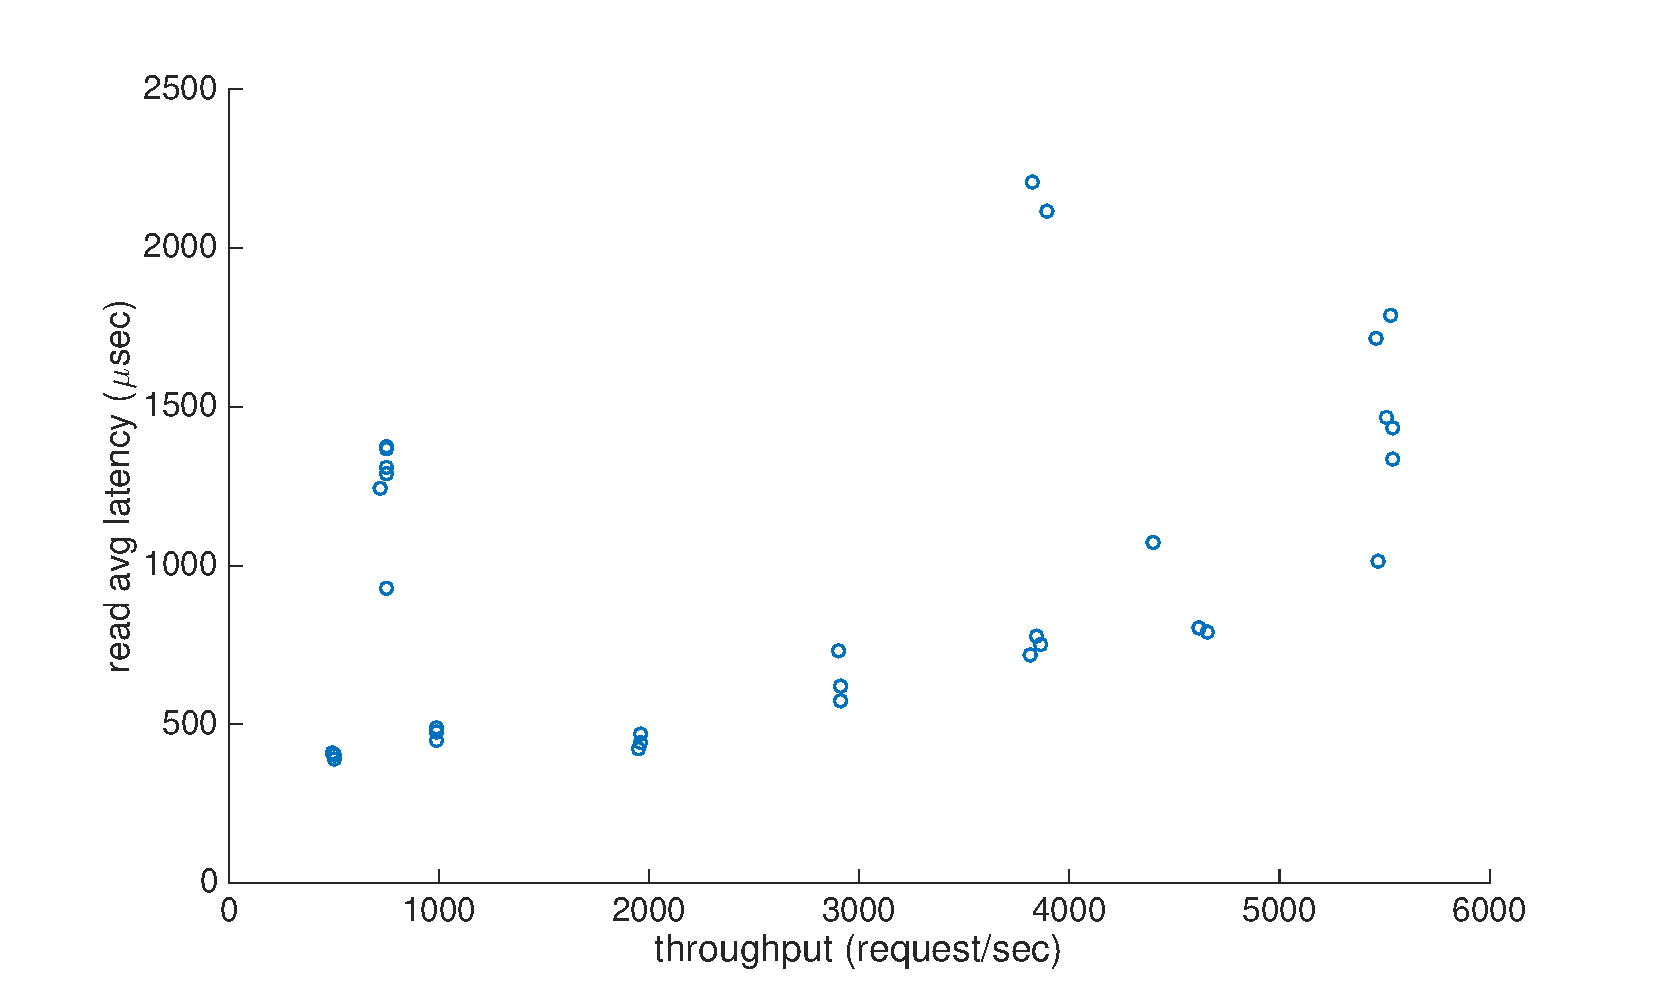
\includegraphics[scale = 0.3]{mysql.eps}
    \caption{Read latency/throughput plot for MySQL}
    \label{figure:mysql}
  \end{figure}
\end{comment}

% \begin{table}
% \centering
% \caption{MySQL $R_{predicted}^2$ for $VM_6$}
% \begin{tabular}{|r|r|l|} \hline
% $R_{read}^2$&$R_{write}^2$&Training Data\\ \hline
% 0 & 0& $VM_1,VM_2,VM_3$\\ \hline
% 0 & 0& $VM_1,VM_2,VM_3,VM_4$\\ \hline
% 0 & 0& $VM_1,VM_2,VM_3,V_4,V_5$\\ \hline
% \hline\end{tabular}
% \label{table:mysql}
% \end{table}